\documentclass[]{article}
\usepackage[margin={.5in, 1in}]{geometry} 
\usepackage{grid-system, graphicx}
\usepackage{cmbright}
\usepackage{grffile}

\newcommand{\plotpath}[1]{{../plots_oberbayern_NEWDATA_MAXPOP5000/#1}.pdf}
\newcommand{\plotwidth}{.8\textwidth}
\newcommand{\plotrow}[2]{\begin{Row}
		\begin{Cell}{1}%
%			\centering
			\includegraphics[width=\plotwidth]{\plotpath{#1}}%
		\end{Cell}%
		\begin{Cell}{1}%
			\if\relax\detokenize{#2}\relax
			\else
%			\centering
			\includegraphics[width=\plotwidth]{\plotpath{#2}}%
			\fi
		\end{Cell}
	\end{Row}
}

\setcounter{section}{-1}

\begin{document}

\begin{center}
	\Huge \textbf{Statistischer Vergleich Engelsbergs mit Gemeinden im Regierungsbezirk Oberbayern mit höchstens 5000 Einwohnern}
\end{center}
\pagebreak

\renewcommand{\contentsname}{Inhalt}
\tableofcontents

\section{Erläuterungen}
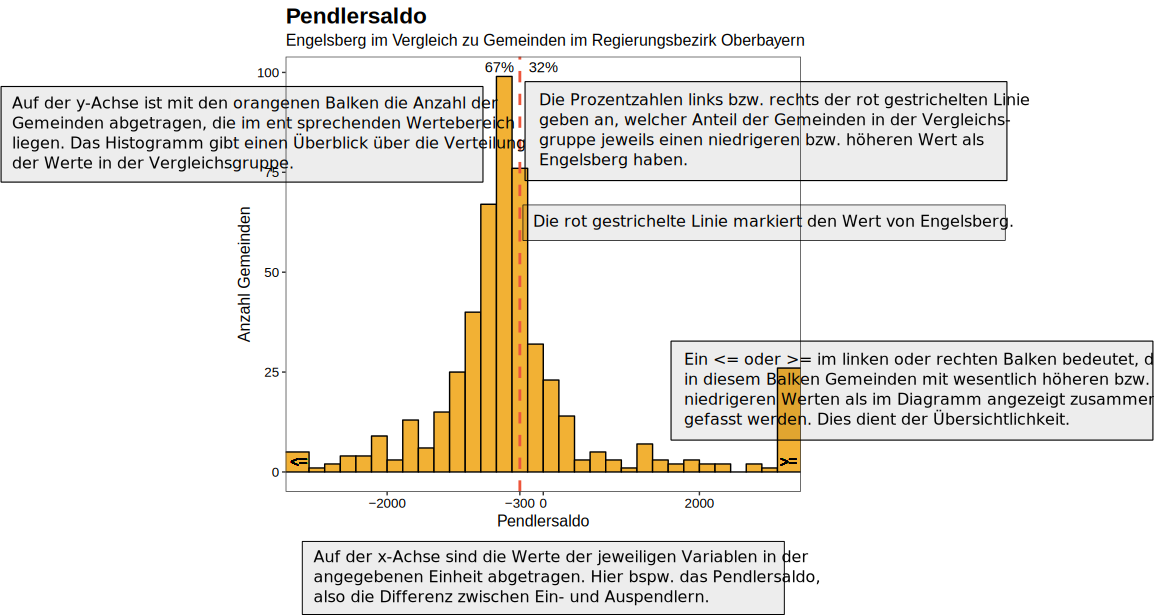
\includegraphics[width=\textwidth]{../plot_explanations}

\vfill

\subsection*{Bevölkerung}
Dieser Vergleich ist auf Gemeinden mit einer Bevölkerung von 5000 oder niedriger beschränkt, um eine bessere Vergleichbarkeit mit Engelsberg zu gewährleisten. Allein die Darstellung der Gesamtbevölkerung (Bevölkerung 2015, Seite \pageref{plot:bevoelkerung.insgesamt}) basiert auf allen Gemeinden.

\subsection*{Quellenangaben}
Alle Diagramme basieren auf verarbeiteten Daten aus Gemeindedaten für Bayern 2018. Ausgewählte statistische Daten für Regierungsbezirke, kreisfreie Städte und Landkreise, Gemeinden und Verwaltungsgemeinschaften sowie Regionen, \textit{Bayerisches Landesamt für Statistik} (2018).

Sofern nicht anders angegeben, beruhen alle Daten auf dem \textbf{Kalenderjahr 2017}.


\section{Bevölkerung}
	\addcontentsline{toc}{subsection}{Bevölkerung insgesamt}
	\addcontentsline{toc}{subsection}{Bevölkerungsdichte}
	\label{plot:bevoelkerung.insgesamt}
	\plotrow{bevoelkerung.insgesamt}{bevoelkerung.je_km2}
	
	\addcontentsline{toc}{subsection}{Bevölkerungsveränderung im Vgl. zu 1987}
	\addcontentsline{toc}{subsection}{Bevölkerungsveränderung im Vgl. zu 2011}
	\plotrow{bevoelkerung.veraenderung.vs.1987}{bevoelkerung.veraenderung.vs.2011}
	
	\addcontentsline{toc}{subsection}{Bevölkerungsbewegung: Zugezogene}
	\addcontentsline{toc}{subsection}{Bevölkerungsbewegung: Fortgezogene}
	\plotrow{bevoelkerung.bewegung.zugezogene}{bevoelkerung.bewegung.fortgezogene}
	
	\addcontentsline{toc}{subsection}{Bevölkerungsbewegung: Wanderungsgewinn}
	\addcontentsline{toc}{subsection}{Bevölkerung: Altersstruktur}
	\plotrow{bevoelkerung.bewegung.wanderungsgewinn}{altersstruktur}

\section{Flächen}
	\addcontentsline{toc}{subsection}{Anteil Gebäude- und Freifläche}
	\addcontentsline{toc}{subsection}{Anteil Betriebsfläche}
	\plotrow{gebfreifl.rel}{betrfl.rel}
	
	\addcontentsline{toc}{subsection}{Anteil Landwirtschaftsfläche}
	\addcontentsline{toc}{subsection}{Anteil Waldfläche}
	\plotrow{landwfl.rel}{waldfl.rel}
	
	\addcontentsline{toc}{subsection}{Anteil Erholungsfläche}
	\plotrow{erholfl.rel}{}

\section{Wohnen}
	\addcontentsline{toc}{subsection}{Wohnungsbestand}
	\addcontentsline{toc}{subsection}{Baugenehmigungen für Wohnungen}
	\plotrow{bauwohn.bestand_wohnungen.insgesamt}{bauwohn.baugenehmigungen.wohnungen}

\section{Kinderbetreuung und Bildung}
	\addcontentsline{toc}{subsection}{Kindertagesplätze}
	\addcontentsline{toc}{subsection}{Schüler}
	\plotrow{bildung.kindertages.plaetze.pro100}{schueler.insg.rel}

\section{Landwirtschaft und Umwelt}
	\addcontentsline{toc}{subsection}{Land- und forstwirtschaftliche Betriebe}
	\addcontentsline{toc}{subsection}{Wasserverbrauch pro Kopf}
	\plotrow{landforst.betriebe_von_flaeche_ha.insgesamt}{umwelt.wasser_pro_kopf_verbrauch}

\section{Erwerb, Einkommen und Soziales}
	\addcontentsline{toc}{subsection}{Beschäftigte am Arbeitsort}
	\addcontentsline{toc}{subsection}{Beschäftigte am Arbeitsort, darunter Einpendler}
	\plotrow{erwerb.sozialverspfl_beschaeftigte_am_arbeitsort.insgesamt}{erwerb.sozialverspfl_beschaeftigte_am_arbeitsort.darunter_einpendler.prozent}
	
	\addcontentsline{toc}{subsection}{Beschäftigte am Wohnort, darunter Auspendler}
	\addcontentsline{toc}{subsection}{Pendlersaldo}
	\plotrow{erwerb.sozialverspfl_beschaeftigte_am_wohnort.darunter_auspendler.prozent}{erwerb.pendlersaldo}
	
	\addcontentsline{toc}{subsection}{Bruttolohn je Arbeitnehmer}
	\addcontentsline{toc}{subsection}{Lohn- und Einkommensteuer: Gesamtbetrag der Einkünfte}
	\plotrow{lohneinksteuer.bruttolohn.je_arbeitnehmer}{lohneinksteuer.gesamtbetrag_einkuenfte.insgesamt}
	
	\addcontentsline{toc}{subsection}{Lohn- und Einkommensteuer: Einkünfte je Steuerpflichtiger}
	\addcontentsline{toc}{subsection}{Sozialhilfeempfänger}
	\plotrow{lohneinksteuer.gesamtbetrag_einkuenfte.je_steuerpfl}{sozialhilfe_empf.insg.rel}

\section{Kommunale Finanzen}
	\addcontentsline{toc}{subsection}{Gemeindesteuereinnahmen: Grundsteuer A}
	\addcontentsline{toc}{subsection}{Gemeindesteuereinnahmen: Grundsteuer B}
	\plotrow{kommunale_finanzen.gemeindesteuereinnahmen.darunter.grundsteuer.a}{kommunale_finanzen.gemeindesteuereinnahmen.darunter.grundsteuer.b}
	
	\addcontentsline{toc}{subsection}{Steuereinnahmen insgesamt}
	\addcontentsline{toc}{subsection}{Gemeindesteuereinnahmen insgesamt}
	\plotrow{kommunale_finanzen.steuereinnahmen_insgesamt}{kommunale_finanzen.gemeindesteuereinnahmen.insgesamt}
	
	\addcontentsline{toc}{subsection}{Steuereinnahmekraft je Einwohner}
	\addcontentsline{toc}{subsection}{Realsteueraufbringungskraft}
	\plotrow{kommunale_finanzen.steuereinnahmekraft.je_einwohner}{kommunale_finanzen.realsteueraufbringungskraft}

\end{document}

%\begin{Row}
%	\begin{Cell}{1}
%		\includegraphics[width=\plotwidth]{\plotpath{}}
%	\end{Cell}
%	\begin{Cell}{1}
%		\includegraphics[width=\plotwidth]{\plotpath{}}
%	\end{Cell}
%\end{Row}
